\mysubsectionformatted{Database Mapper - Indirect Mapping}
\myparagraph{
    \begin{tcolorbox}[colback=blue!5!white, colframe=blue!75!black]
        Il framework (o pattern di progettazione) permette di definire una classe che si occupi della gestione dei processi
        di materializzazione da un DB, la dematerializzazione della memoria verso il DB e
        il caching degli oggetti con l'obiettivo di aumentare la performance del sistema.
    \end{tcolorbox}

    Il pattern definisce un DB Mapper per ogni classe di oggetti persistenti, possono esistere diversi
    tipi di Mapper a seconda dei meccanismi di memorizzazione.

    \begin{center}
        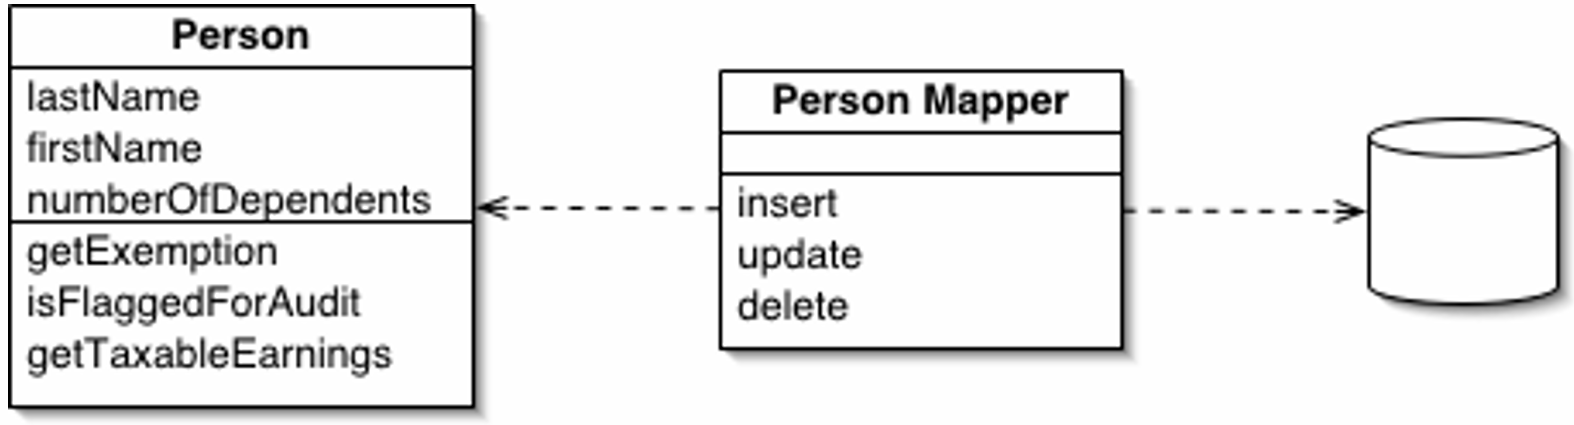
\includegraphics[scale=0.25]{Esercitazione - Design Patterns/Database Mapper.png}
    \end{center}

    \textbf{Person Mapper} è uno strato separato di componenti dedicati a trasferire i dati fra l'applicazione
    (\textbf{Person}) e il \textbf{Database}, trattando indipendentemente i due schemi (OO e ER). Infatti, la
    logica di business è inconsapevole dell'esistenza del Database.\\
    Generalmente, il pattern ne coinvolge di ulteriori per la gestione della sincronizzazione fra i due schemi
    (es. \textit{UnitOfWork} o \textit{IdentityMap}).\\
    Usiamo questo pattern per \textbf{gestire un mapping complesso fra DB e logica di business}.

    \begin{center}
        \resizebox{\columnwidth}{!}{%
            \begin{tabular}{ll}
                \hline
                \rowcolor[HTML]{32CB00}
                \multicolumn{1}{|c|}{\cellcolor[HTML]{32CB00}\textbf{Vantaggi}} & \multicolumn{1}{c|}{\cellcolor[HTML]{FE0000}\textbf{Svantaggi}} \\ \hline
                \multicolumn{1}{|l|}{Isola totalmente i due strati}             & \multicolumn{1}{l|}{Difficolta nell'implementazione}            \\ \hline
                                                                                &
            \end{tabular}%
        }
    \end{center}
    \newpage
}